\section{Scenario B: Email Digest}
In the Email Digest Scenario, we will identify a batch of up to 100 ranked tweets per day per interest profile.At a high level, these results should be relevant and novel; timeliness is not important as long as the tweets were all posted on the previous day.

As shown in \ref{fig:Bsys}, our system for this scenario mainly contains four modules:

\begin{itemize}
\item \textbf{Data cleaning module:} We pre-process all tweets during evaluation period. And we simply filter tweets that do not contain any keywords for each interest profile, and the rest tweets are chosen as candidate tweet collection, which will accelerate identifying possible relevant tweets for each profile.

\item \textbf{Query expansion module:} As microblog retrieval suffers severely from the
vocabulary-mismatch problem (i.e. term overlap between query and tweet is relatively small). To tackle this issue, we leverage web-based query expansion method to improve retrieval performance. As is known to all, Google search is the dominant search engine in the majority countries over the world, which indexes billions[195] of web pages, so that users can search for the information they desire through the use of keywords and operators. Therefore, we take the interest profile as the keywords to search in Google with Google Search Engine API before the evalution period.


As the user interest profile offered by TREC 2016 are JSON-formatted structure and each profile includes four fields, topid, title, description and narrative. Here we only use the topic keywords as our \emph{OriginQuery} since we utilize external web resource to depict the background information, noted as \emph{IssueQuery}. Then, we generate the \emph{ExpansionQuery} by interpolating the \emph{OriginQuery} and \emph{IssueQuery}.

\begin{equation}
\label{equ:merge}
\emph{ExpansionQuery} = \alpha \cdot \emph{OriginQuery} + (1-\alpha) \cdot \emph{IssueQuery}
\end{equation}

We utilize the expanded query to represent the interest profile and then estimate the relevance between the query and tweets.

\item \textbf{Relevance ranking module:} Similar with Scenario A, we utilize the KL-divergence language model based retrieval method to measure the relevance between query and tweet.

\item \textbf{Novelty verfication module:} Once we obtain the ranked tweet list after relevance ranking, we adopt the novelty verfication module along with pushed tweet pool to pick up novel tweets.


In this module, there are two kinds of strategies to measure novelty between tweets: (1)Language model. The higher relevance score between tweets, the less novelty they are. (2)Simhash, which is a popular method to handle web page redundancy. simhash is one where similiar items are hashed to similiar hash values and we can calculate the bitwise hamming distance between hash values. The closer hamming distance between two tweets is, the more similar they are. The simhash code is calculated as follow,

****公式
\end{itemize}

\begin{figure}[htbp]
\centering
{
	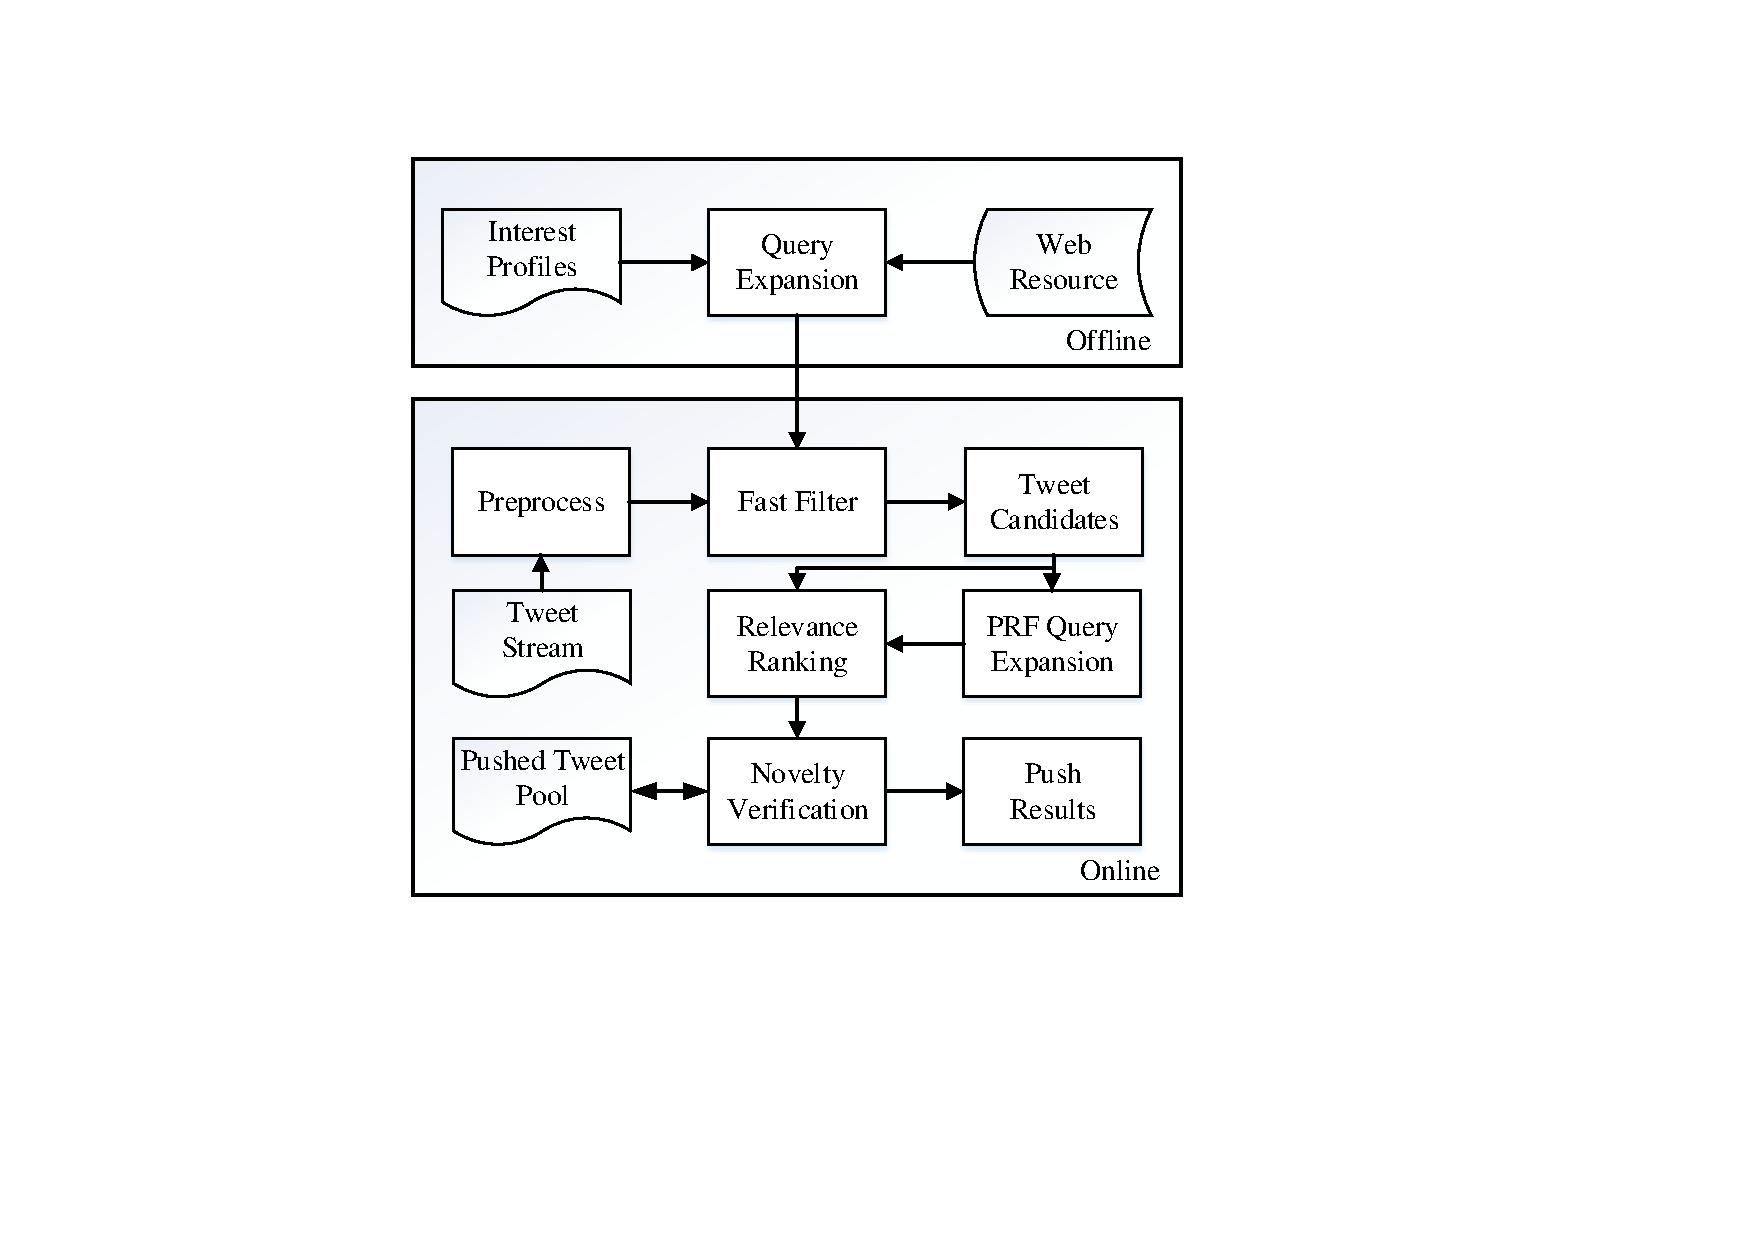
\epsfig{file=figures/scenarioB.pdf,width=0.45\textwidth}
}
\caption{Scenario B System Framework.}
\label{fig:Bsys}
\end{figure}


% In this section, we first introduce the preliminaries and then present our approach.
% The proposed approach is a combination between an embedding based model and a probabilistic retrieval ranking method. Our major focus is to extend the traditional embedding model for the current task. The extensions are in two aspects: (1) We incorporate supervised labels in the embedding models; (2) We automatically rank candidate phrases to generate pseudo functional labels.

% \subsection{Preliminaries}
% Let $d$ denote a business and $w$ denote a word. A business $d$ is associated with a set of reviews which are further combined into a single \emph{review document} $R^{(d)}: w_1,...,w_{N_{d}}$, where $w_i$ denotes the $i$-th word in $R^{(d)}$  and $N_d$ is the length of $R^{(d)}$. We further assume that a business $d$ is also associated with an attribute set $\mathcal{A}^{(d)}$. An attribute $a \in \mathcal{A}^{(d)}$ can denote any useful business attribute, such as business ID, business name and functional labels. A label $l: w_1,..., w_{N_{l}}$ is a phrase (i.e., a word sequence), where $N_{l}$ is the length of label $l$. 

% Given a set of candidate labels $\mathcal{L}$ and a business $d$, we aim to automatically select meaningful labels from  $\mathcal{L}$ for $d$. Currently, we assume that the candidate label set is available by aggregating all the attached historical labels in a domain. We cast the task as a ranking problem by defining a general relatedness score function $S(d,l)$. With some score function $S(\cdot, \cdot)$, we can rank the candidate labels and find the top best $K$ ones for a specific business. Next we will study how to set the score function. %First, we consider the embedding similarity as the score function. 

% \subsection{Measuring the Relatedness Using Okapi BM25}
% Since we have formulated the current task as a ranking problem, any relevance measurement method can apply here. By borrowing the techniques in Information Retrieval, we adopt the classic probabilistic retrieval ranking model, i.e., Okapi BM25 \cite{bm25-1,bm25-2} to capture the lexical similarity. We present the Okapi BM25 model in our task setting as follows

% \begin{tiny}
% \begin{equation}\label{eq-bm25}
% S_{BM25}(d,l)=\sum_{w \in l} IDF(w)\cdot \frac{f(w,d)\cdot(k_1+1)} {f(w,d)+k_1\cdot(1-b+b\cdot\frac{N_d} {avgdl)})}
% \end{equation}
% \end{tiny}

% where $f(w,d)$ is the term frequency of $w$ in $R_d$, $avgdl$ is the average review document length in the data collection, $k_1,b$ are tuning parameters and $IDF(w)$ is inverse document frequency of the term $w$,  defined as

% \begin{equation*}
% IDF(w)=\log\frac{N-n(w)+0.5} {n(w)+0.5}
% \end{equation*}

% where $N$ is the total count of business in the collection, and $n(w)$ is the number of review documents contains $w$.



% \subsection{Measuring the Relatedness Using an Attribute-based Semantic Embedding Model}
% \label{sec:method}
% The classic Okapi BM25 model performs well in practice, however, it only captures the similarity based on shallow term semantics. We now study how to derive similarity measurement based on latent embedding semantic space. 
% Inspired by distributed representation methods \cite{word_to_vector}, we propose a general attribute-based semantic embedding model, which projects both attributes and words into the low-dimensional semantic space.  



% \subsubsection*{Defining the Objective Function} 
% As mentioned above, a business $d$ is associated with a review document $R^{(d)}$ and an attribute set $\mathcal{A}^{(d)}$.  Our main idea is to maximize the generative likelihood of the review document based on the attribute set. Formally we define the following objective function \footnote{For simplicity, we will only present the objective function for a single business, it will be easy to extend to multiple businesses.}

% \begin{equation*}
% \frac{1} {N_{d}} \sum_{i=1}^{N_{d}} \log Pr(w_i|w_{i-c}:w_{i+c}, \mathcal{A}^{(d)}),
% \end{equation*}

% where $w_{i-c}:w_{i+c}$ is the subsequence $(w_{i-c},\ldots,w_{i+c})$ by excluding $w_i$ and $2\times c$ is the window size. The generative story can be summarized as follows: each word is generated with the context of its surrounding words in the review document and the business-specific attribute set.  We model both words $w_i$ and attributes $a_j$ as an $M$-dimensional embedding vector $\bm{v}_{w_i}$ and  $\bm{v}_{a_j}$ respectively. With this form of embedding representation, we further employ a multiclass classifier softmax to formulate the probability $Pr(w_i|w_{i-c}:w_{i+c}, \mathcal{A}^{(d)})$ as follows

% \begin{equation*}
% Pr(w_i|w_{i-c}:w_{i+c}, \mathcal{A}^{(d)}) =\frac{\exp(\bar{\bm{v}}_{w_i}^\mathrm{\top}\bm{v}^{\prime}_{w_i})} {\sum_{w \in \mathcal{W}} \exp(\bar{\bm{v}}_{w}^\top \bm{v}_w^\prime)}
% \end{equation*}

% where $\mathcal{W}$ is the word vocabulary, $\bm{v}_{w_i}^\prime$ is the output vector representation of target word $w_i$ and  $\bar{\bm{v}}_{w_i}$ is the averaged vector representation of the context defined below

% \begin{equation*}
% \bar{\bm{v}}_{w_i}=\frac{1} {2c+|\mathcal{A}^{(d)}|} (\sum_{-c \leq k \leq c,k \ne 0}\bm{v}_{w_{i+k}}+\sum_{a_j \in \mathcal{A}^{(d)}}\bm{v}_{a_j}).
% \end{equation*}


% \subsubsection*{Construction of the Attribute Set} 
% Previously, we presented a general attribute-based embedding model, which jointly considers word contexts and business-attribute contexts for representation learning. This model is general since it is flexible to incorporate any useful business attributes.  In practice, many attributes 
% can be used, including business type, open hour, rating star and location. In our work, our aim is to derive a similarity measurement between a business and a candidate label. Based on this point, we consider three kinds of specific attributes.

%  \emph{Business ID:} We simply put a business ID into its corresponding attribute set. In this way, we can learn an embedding representation $\bm{v}_d$ for a business ID $d$.

%  \emph{Business Name:} A business name usually reflects the main characteristics of the corresponding business. For a business, we treat all the words in the business name as the attributes. 

%  \emph{Pseudo Labels:} We incorporate pseudo labels into the corresponding attribute set. In our task, we assume that there is no supervised information provided to the algorithm, and there are no gold labels available in the training set.  As motivated in Section 1, the review text tends to contain important evidence for the candidate functional labels, so we try to automatically leverage pseudo labels from review text. The learnt labels do not necessarily match with the gold labels, that is why we call them ``pseudo labels". We would like to utilize such weak supervision information to guide the learning process for semantic embedding. 
%  The key point is how to select pseudo labels. A straightforward way is to rank the candidate labels in $\mathcal{L}$ with the number of occurrences in review text. However, the exact surface match might not work well due to the fact that reviews contain noise, misspelling and slang. So we propose to use the Okapi BM25 model in Eq.~\ref{eq-bm25} to select pseudo labels.  In other words, only the top ranked labels derived will be considered as pseudo labels. Our main assumption is that the highly ranked pseudo labels are implicit labeled information conveyed by the users.  If a large amount of users have indicated the importance and relatedness of a label in their own reviews, it should be a good candidate functional label. By leveraging such collective knowledge, the embedding model is more capable of learning the semantics for the functional labels. 

% \subsubsection*{Defining the Embedding Score Function}

% We adopt the commonly used Stochastic Gradient Descent (SGD) for parameter learning and use Back-Propagation for gradient update. Once the model is well learnt, we can obtained the corresponding representations for words, business IDs and pseudo labels \footnote{Business names are broken into words, and we do not set up specific representations.}. For ranking the candidate labels, we use the inner product to measure the relatedness between a business $d$ and a label $l$


% \begin{equation}\label{eq-embedding}
% S(d, l)_{E} = \bm{v}_{d}^{\top} \cdot \bm{v}_{l}.
% \end{equation}

% where we assume that a candidate label set $\mathcal{L}$ is given, and we can learn an embedding representation $\bm{v}_l$ for a candidate label $l$  \footnote{Note if there exists a label $l' \in \mathcal{L}$ never selected as a pseudo label for all the businesses, we will aggregate (i.e., average) the corresponding embedding vectors of the words in the label as its final representation.}.

% \subsection{Combining Lexical Similarity and Embedding Similarity}

% Lexical similarity captures term-based semantic similarity, while embedding similarity measures the relatedness in the embedded low-dimensional semantic space.  We combine these two kinds of similarities to characterize the semantic relatedness in a more comprehensive way.


% \begin{equation}
% S(d, l) = \lambda \times S(d, l)_{BM25} + (1-\lambda) \times S(d, l)_{E},
% \end{equation}

% where $S(d, l)_{BM25}$ and $S(d, l)_{E}$ are scoring functions defined in Eq.~\ref{eq-bm25} and \ref{eq-embedding} respectively, and  $\lambda$ is a parameter falling in $(0,1)$ to tune. 

